\documentclass[whitelogo]{tudelft-report}
\usepackage{natbib}
\usepackage{changes}
\usepackage{amsmath,bm}
\usepackage{braket}
\usepackage{wrapfig}
\usepackage{caption}
\usepackage{subcaption}
\usepackage{amssymb}
\usepackage{graphicx}
\usepackage{physics}
\usepackage[utf8]{inputenc}
\DeclareMathAlphabet{\mathcal}{OMS}{cmsy}{m}{n}
\newcommand*\Laplace{\mathop{}\!\mathbin\bigtriangleup}

\begin{document}

%% Use Roman numerals for the page numbers of the title pages and table of
%% contents.
%\frontmatter

%% Uncomment following 19 lines for a cover with a picture on the lower half only
%\title[tudelft-white]{Title}
%\subtitle[tudelft-cyan]{Optional subtitle}
%\author[tudelft-white]{J.\ Random Author}
%\affiliation{Technische Universiteit Delft}
%\coverimage{cover.jpg}
%\titleoffsetx{10cm}
%\titleoffsety{10cm}
%\afiloffsetx{1cm}
%\afiloffsety{18cm}
%\covertext[tudelft-white]{
%    \textbf{Cover Text} \\
%    possibly \\
%    spanning 
%    multiple 
%    lines
%    \vfill
%    ISBN 000-00-0000-000-0
%}
%\makecover

%% Uncomment following 16 lines for a cover with a picture on the lower half only
\title[tudelft-black]{Design of a trijunction of Majorana nanowires}
%\subtitle[tudelft-black]{Optional subtitle}
\author[tudelft-black]{Juan Daniel Torres Luna}
\affiliation{Technische Universiteit Delft}
%\coverimage{tank.jpg}

\setpagecolor{tudelft-cyan}
\makecover[split]


%% Include an optional title page.
\begin{titlepage}


\begin{center}

%% Insert the TU Delft logo at the bottom of the page.

%% Print the title in cyan.
{\makeatletter
\largetitlestyle\fontsize{40}{94}\selectfont\@title
%\largetitlestyle\color{tudelft-cyan}\Huge\@title
\makeatother}

%% Print the optional subtitle in black.
{\makeatletter
\ifx\@subtitle\undefined\else
    \bigskip
   {\tudsffamily\fontsize{22}{32}\selectfont\@subtitle}    
    %\titlefont\titleshape\LARGE\@subtitle
\fi
\makeatother}

\bigskip
\bigskip

by
%door

\bigskip
\bigskip

%% Print the name of the author.
{\makeatletter
%\largetitlefont\Large\bfseries\@author
\largetitlestyle\fontsize{26}{26}\selectfont\@author
\makeatother}

\bigskip
\bigskip

to obtain the degree of Master of Science
%ter verkrijging van de graad van Master of Science

at the Delft University of Technology,
%aan de Technische Universiteit Delft,

to be defended publicly on April 21st
%in het openbaar de verdedigen op dinsdag 1 januari om 10:00 uur.

\vfill

\begin{tabular}{lll}
    Student number: & 5213983 \\
    Project duration: & \multicolumn{2}{l}{August 31, 2021 -- March 2, 2022} \\
    Thesis committee: & Prof. Michael Wimmer, & TU Delft, supervisor \\
        & Prof. Anton Akhmerov & TU Delft, co-supervisor \\
        & Dr. Chun-Xiao Liu & TU Delft, co-supervisor
\end{tabular}
%% Only include the following lines if confidentiality is applicable.

\bigskip
\bigskip
%\emph{This thesis is confidential and cannot be made public until December 31, 2013.}
%\emph{Op dit verslag is geheimhouding van toepassing tot en met 31 december 2013.}

\bigskip
\bigskip
%An electronic version of this thesis is available at \url{http://repository.tudelft.nl/}.
%\\[1cm]

%\centering{
\includegraphics{cover/logo_black}}


\end{center}

\begin{tikzpicture}[remember picture, overlay]
    \node at (current page.south)[anchor=south,inner sep=0pt]{
        
\includegraphics{cover/logo_black}
    };
\end{tikzpicture}

\end{titlepage}

%\input{chapters/preface}

\tableofcontents

%% Use Arabic numerals for the page numbers of the chapters.
\mainmatter


\chapter{Background}

\section{Introduction}

Majorana bound states (MBS) can be used to store quantum information protected from the local environment.
MBS can be realised in a hybrid quasi-one dimensional system that combines a strong-spin orbit semiconductor with proximity induced superconductivity.
Semiconducting nanowires and two-dimensional electron gases (2DEG) are candidates for creating such devices.

Majorana based quantum computation requires controlled interaction of multiple MBS in a two dimensional device.
The ground state evolves following controlled quantum operations by selectively coupling different MBS pairs.
Nanowires networks or gate-defined networks in 2DEGs have been studied experimentally and theoretically as platforms for Majorana based computation.

While coupling a single MBS pair can be done using a quantum dot, selective coupling of multiple pairs remains a challenge.
On one hand, there are geometrical constraints given by tuning multiple separate nanowires in the topological phase.
On the other hand, the coupling of multiple pairs should be optimised simultaneously by the device geometry.
Therefore, design and operate a multi Majorana device is a non-trivial task.
 
The simplest system where multiple MBS can couple non-trivially is in a trijunction geometry.
In this thesis we propose a semiconducting cavity connected to three Majorana nanowires that allows for an all-electric controlled interaction between all pairs of MBS.

Initially, the role of geometry is investigated by simulating several cavity geometries and extracting the MBS coupling in the strong coupling regime.
We found that the geometrical configuration of the trijunction modulates the coupling of the MBS pairs.
Several cavity geometries are analysed, and a triangular cavity with varying angle is found to have the largest coupling for all pairs simultaneously.

Finally, a realistic model is studied via electrostatic simulations of a gate-defined triangular configuration defined on a 2DEG.
The non-local nature of the gates makes the nanowire positions crucial in order to recover the effects found for the purely geometric case.
The role of each set of gates and the range of voltages used to operate the device are discussed.
The electrostatics effects of the gate-defined triangular cavity are analysed and the operational point is described.


\section{Majorana bound states}

\begin{figure}[h!!]
\centering
  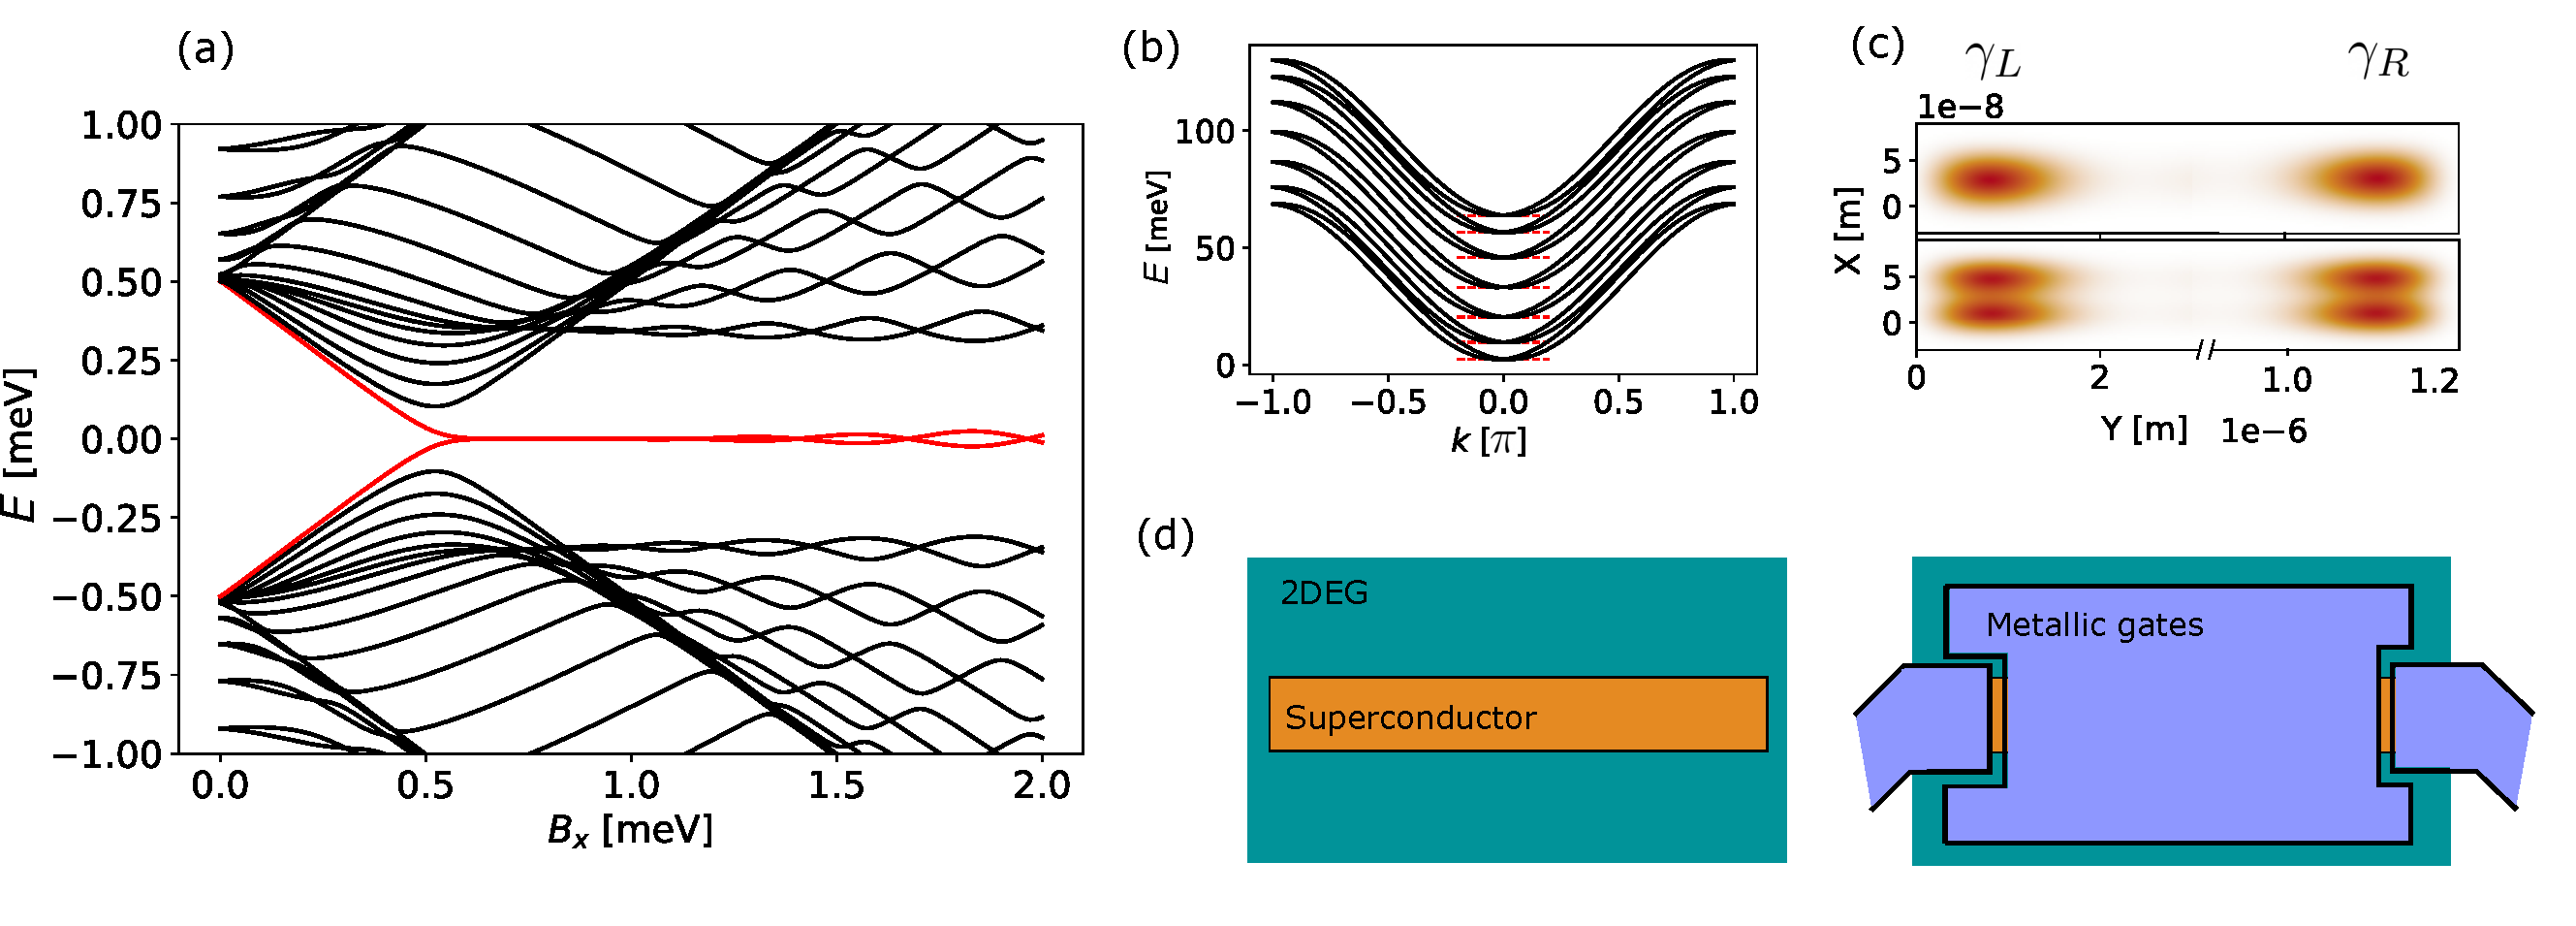
\includegraphics[width=0.95\linewidth]{figures/majorana_intro.pdf}
  \caption{Simulations of a Majorana nanowire as described in Eq. \eqref{eq:ham_maj}. The following parameters will be used in all simulations:  $\Delta=0.5$[meV], $\alpha=0.3$[eV A], and $m^*=0.023 m_e$. Each simulated nanowire has length $L=120*a$ and width $W=7*a$ where $a=10$[nm] is the lattice constant size. (a) Topological phase transition as a function of Zeeman field $B_x$. Lowest mode (red) sticks to zero after crossing the critical field. (b)  Transverse bands along the translational invariant direction with $\Delta=0$. The chemical potential is tuned to the bottom of each band (red dashed lines) to create Majoranas. (c) Majorana wavefunctions for the lowest two bands. (d) Illustration of how a Majorana nanowire is built on a 2DEG. Left panel shows the 2DEG with a superconducting stripe on top. Right panel shows the system after the deposition of the gates.}
  \label{fig:intro}
\end{figure}

MBS populate the non-local degenerate ground state of a topological superconductor\cite{Alicea2011}.
Under the appropriate conditions, a spinless one-dimensional $p$-wave superconductor contains two zero-energy excitations that are exponentially localised at the edges of the system. 
Together, these two zero-energy modes encode a single fermionic mode that can be empty or occupied, 
\begin{equation}
f = \frac{\gamma_{L} + i\gamma_{R}}{\sqrt{2}}, \quad f^{\dagger} = \frac{\gamma_{L} - i \gamma_{R}}{\sqrt{2}},
\end{equation}
where $\gamma_{i} = \gamma_{i}^{\dagger}$ are Majorana operators that satisfy $\{ \gamma_{i}, \gamma_{j} \} = 2\delta_{ij}$.
%The ground state $\ket{\Psi}$ is two-dimensional, and it is spanned by the states $\ket{0}$ and $f^{\dagger}\ket{0}$, i.e. empty and occupied states.

%\textit{Since a pair of spatially separated MBS encode a single fermionic mode, its quantum state is protected against local errors by particle-hole symmetry.}
In a sufficiently long nanowire, MBS are decoupled from each other, and noise sources will interact with each of them individually.
The interaction with a single MBS is proportional to a single Majorana operator, i.e. $\gamma \sim f + f^{\dagger}$, and thus it will change the parity of the system.
In a superconductor, however, electrons can only enter or leave as Cooper pairs, which means that the parity is conserved. 
Therefore, individual MBS are immune to local noise sources.

Consequently, only even powers of Majorana operators are allowed in the Hamiltonian.
The simplest allowed term describes the coupling of a pair of MBS.
In a single nanowire, or in a linear array of them, it is only possible implement this term with successive MBS.
It is given by,
\begin{equation}\label{eq:H_pair}
H_{pair} = i E_{LR} \gamma_{L} \gamma_{R} = E_{LR} (1 - 2 f^{\dagger} f).
\end{equation}
Here, $E_{LR}$ is the tunnelling coupling between the two MBS.
Consequently, a general state within the degenerate subspace evolves as,
\begin{equation}
\ket{\Psi}  = \alpha \ket 0 +\beta \ket 1 \rightarrow U(t) \ket{\Psi} = \alpha \ket 0 + \beta e^{2 i E_{LR} t} \ket 1.
\end{equation}
%\textit{The ground state can only evolve by non-local operations that involve pairs of MBS.}

However, universal quantum computation cannot be built from using only quadratic fermionic terms as in Eq. \ref{eq:H_pair}.
Controlled interaction between MBS from different fermions are essential to Majorana based quantum computation\cite{Sau2011, Leijse2021, Bauer2018}.
Therefore, a higher dimensional structure where multiple MBS converge is required in order to do Majorana computation.
%In the presence of multiple MBS pairs, on the other hand, each parity subspace can be used as a computational subspace.
%\textit{By controlling the coupling between different MBS pairs, one can control the ground state evolution}, that is,

\section{Experimental platforms}

%MBS were only in Kitaev's toy model until several proposals for realising them on solid-state devices appeared.
%The main problem was that electrons are not spinless, and $p$-wave superconductor have not been found so far.
%Superconductors pair electrons with different spins, i.e. singlets, as suggested by BCS theory.
%However, by combining a $s$ wave-superconductor, such as Al, and a material with strong spin orbit coupling, such as $InAs$ or $InSb$, one can effectively realise spinless fermions in the presence of a magnetic field.
%However, creating such material combination 
\textit{MBS can be realised in quasi one-dimensional systems defined on two-dimensional electron gases (2DEGs), or semiconducting nanowires, with strong spin-orbit and in proximity to a superconductor.}
The Hamiltonian that realises a Majorana nanowire\cite{Alicea2011} is,
\begin{equation}\label{eq:ham_maj}
\mathcal{H} = \sum_k \Psi_k^\dagger H(k) \Psi_k  ,\quad H(k) =  \left[ \frac{|\mathbf{k}|^2}{2 m^*} - \mu + \alpha(k_x \sigma_y - k_y \sigma_x) \right] \tau_z + B_x \sigma_x  + \Delta \tau_x.
\end{equation}
Here, $\Psi_k^\dagger = (f_{k\uparrow}^\dagger, f_{k\downarrow}^\dagger, f_{k\uparrow} f_{k\downarrow})^T$ are the Nambu spinors in $k$ space, $\mu$ is the chemical potential, $\mathbf{k}$ is the 2D wave-vector, $\alpha$ is the spin orbit interaction, $B_x$ is the Zeeman field, $\Delta$ is the superconducting gap, and $\sigma$ and $\tau$ are Pauli matrices for the spin and particle-hole basis.
MBS appear as zero energy excitations of this Hamiltonian when $B_x^2 \geq \sqrt{\mu^2 + \Delta^2}$.

\textit{Realising such material combination is a challenge, and MBS transport signatures are not unambiguous\cite{Vuik2019,Liu2018}.}
For example, superconductivity and magnetic fields compete with each other.
On the other hand, MBS signatures can be reproduced by states localised in material defects or impurities.
Consequently, most of the current work in this field is focused on unambiguously finding a single MBS pair.

Truly one-dimensional systems do not exist.
There is a translational invariant direction, and at least one direction with finite width $W$.
The energy of each mode has a contribution from both, and it is given by,
\begin{equation}
E_{n}(k) = \frac{\hbar^{2}}{2m^*} \left( k^{2} + \frac{\pi^{2} n^{2}}{W^{2}} \right).
\end{equation}
Here, $m^{*}$ is the effective mass and the spin orbit splitting is not considered.
Independent MBS with different momentum profiles can be formed at each transverse mode when the chemical potential is at the bottom of the corresponding band\cite{Reeg2018}.

%Multiple channel become relevant in the presence of disorder.
%It couples differently to each momentum sub band, which will induce band mixing as has been suggested in experiments.

%\textit{Disorder in the nanowire bulk can be detrimental for MBS since it affects its localisation and properties, such as induced gap, while disorder inside the superconductor enhances the induced gap in the nanowire.}

\subsection{Two dimensional electron gases}

In order to build a multi Majorana device we require a flexible 2D platform where multiple nanowires can be easily attached.
Furthermore, it been shown that properties of Majorana devices can be modulated by changing the device geometry.
\textit{2DEGs appear as an interesting platform for since arbitrary geometries can be created using electrostatic gates.}
On the other hand, high-quality networks of semiconducting nanowires can be built, but geometries are limited to straight configurations.

\textit{Parallel Majorana nanowires are the basic elements for a complex Majorana device.}
A single nanowire on a 2DEG can be created by adding a superconducting strip on top of the selected region as shown in Fig. \ref{fig:intro} (d).
Then, a top gate is deposited next on top of the device such that depletes the surrounding 2DEG.
A narrow quasi-one dimensional channel is created below the superconductor where the gate electric field is screened\cite{Hell2017}.
Following this procedure, multiple parallel nanowires can be created in a 2DEG by selectively depositing superconducting covers.

\textit{There are several Majorana experiments on 2DEGs that have shown promising evidence for scalable and complex devices.}
Initial experiments\cite{Shabani2015,Kjaergaard2016} focused on characterising the properties of semiconducting layers with a superconducting cover.
Advances in material growth allowed for clean interfaces with a hard superconducting gap to develop into the nanowire region.
Later experiments focused on tunnel spectroscopy of stripe-like geometries\cite{Suominen2017} where a zero bias peak (ZBP) was found.
However, due to disorder and defects such ZBPs have most likely a trivial origin from Andreev states rather than MBS.
Nevertheless, efforts to develop complex devices in 2DEGs are made and new promising materials are being studied.

\subsection{Electrostatic gates}

The potential landscape in a 2DEG can be controlled by deposition of metallic gates on a top layer with an insulating barrier in between that smooths the potential profile\cite{Antipov2018}.
\textit{The electrostatic potential in a 2DEG is found by solving the Poisson equation using a finite elements method on the device geometry.}
The potential landscape, $U(\mathbf{r})$, for a given geometrical configuration can be found by solving Laplace equation,
\begin{equation}\label{eq: laplace}
\nabla \cdot \left[ \varepsilon_r(\mathbf{r}) \nabla U(\mathbf{r}) \right] = 0.
\end{equation}
Here, $\varepsilon_r$ is the relative permittivity of each layer in the material stack.
In general, the quantum electrostatics problem is more complicated due to the interaction of dopant charges with the potential.
However, our problem is simpler since no extra charges are required.

%\textit{Electrostatic effects play a crucial role in designing and operating Majorana devices}.
%Characterisation of Majorana nanowire is done via transport measurements that require tunnel coupled leads and gates.
%Furthermore, gates have a non-local effect on the potential landscape that differs between experimental platforms.
%For example, nanowires have a partial superconducting coating that allows for the electric field to penetrate and control the semiconductor and superconductor weight of the wavefunction.
%In 2DEGs, on the contrary, the superconducting coat fully covers it, which screens electrostatic effects.

\section{Majorana bound states in a trijunction}

In order to create a Majorana qubit, at least three MBS with local pair interactions are required\cite{Alicea2011}.
The device that realises this selective coupling is called a trijunction.
It contains two parts: three nanowires, and a central cavity that mediates the coupling.
In such a system, demonstration of the simplest non-trivial Majorana evolution experiment can be done.

The geometrical configuration of the trijunction is subject to two main constraints:
On one hand, nanowires must be parallel since the topological phase closes for small deviations of the magnetic field.
On the other hand, nanowires must have a significant separation from each other such that MBS are well isolated.
Consequently, the design of a trijunction geometry with selective coupling between MBS pair is a non-trivial task.

Previous trijunction designs\cite{Hell2017} have studied MBS coupling in the tunnelling regime.
The trijunction is defined using gates placed on top of a 2DEG, and it is operated by controlling the voltages of the different gates.
In this context, the MBS coupling relies entirely on wavefunction overlap along the cavity. 
Consequently, MBS pairs acquire relatively small couplings with the advantage of not introducing any extra sub gap state.

On the other hand, in the strong coupling the MBS coupling is mediated by cavity states but with extra levels present inside the gap.
Nevertheless, the coupling energy of the MBS pairs can become significantly larger, i.e. comparable with the induced gap.
The modulation of the coupling now relies on the cavity geometry.
Interestingly, it has been shown that properties Majorana devices can be optimised by using geometrical effects.
In this context, this work explores the geometrical dependence of selectively coupling multiple MBS pairs in a Majorana trijunction.

%\textit{There are two main approaches for MBS quantum computation: braiding and joint parity measurements.}
%Braiding was initially proposed as moving MBS around each other in gate defined nanowire networks. 
%However, this method requires high degree of control and is highly susceptible to thermal errors\cite{Pedrocchi2015}.
%On the other hand, joint parity measurements coupling multiple pairs of MBS by using co-tunnelling processes between different MBS on superconducting islands.


%\textit{However, design and operation of a trijunction are non-trivial tasks.}
%Simultaneous tuning of gate voltages and relative phase difference is required to optimally operate a trijunction.
%Selection of the MBS pair and cavity modes is realised by electrostatic gates controlling the potential on each region.
%Furthermore, relative phase differences between MBS modulates the coupling as in the fractional Josephson effect.
%The phase will be shifted by the presence of complex hopping terms and by the nanowires relative position.

%\begin{enumerate}
%\item The dimension of the computational Hilbert space depends on the number of MBS, and thus multiple parallel Majorana nanowires are required for MBS based quantum computing.
%\item 
%\item An equivalent approach that does not require to move the MBS is given by joint parity measurements\cite{Bonderson2008}, but it requires simultaneous measurement of different pairs of MBS.


%\section{Quantum dot mediated coupling}

%\begin{enumerate}
%\item A single nanowire coupled to a quantum dot (QD) allows to measure the parity of a pair of MBS via a measurement of the charge in the dot.
%\item In a single nanowire model, the interaction is controlled by the overlap of the MBS pair which depends on the wire length.
%\item Two nanowires with a QD in the middle recovers the well-know Josephson junction whose spectra can be controlled by the phase difference between the two superconductors.
%\item The fractional Josephson effect, $4\pi$ phase periodicity, is a consequence of the presence of a zero-energy fermionic mode made of two MBS.

%\end{enumerate}


\chapter{Trijunction of Majorana nanowires}

In this chapter we demonstrate that the coupling of three pairs of MBS in a trijuction is determined by the geometrical details of the central semiconducting cavity.
For certain geometrical configurations, a MBS pair couples resonantly with successive cavity states as in the so-called \textit{resonant trapping}, while in other cases the coupling is mediated by individual non-overlapping levels.

The basic operation of the trijunction follows the procedure described in Fig. \ref{fig:tj_example}.
We consider the strong coupling regime where there are no tunnel barriers between the cavity and the nanowires.
The cavity chemical potential is varied in a range of $4$ meV around the first resonance for all cavities.
In this range, there are multiple levels that couple resonantly with a given pair of MBS.
In order to characterise the coupling, we extract the highest resonance peak for each geometry as indicated by the black arrows in Fig. \ref{fig:tj_example} (b).
Then, we classify them according to their operational robustness, that is, height and width.

\section{Quasi-one dimensional cavities}

\begin{figure}[h!]
\centering
  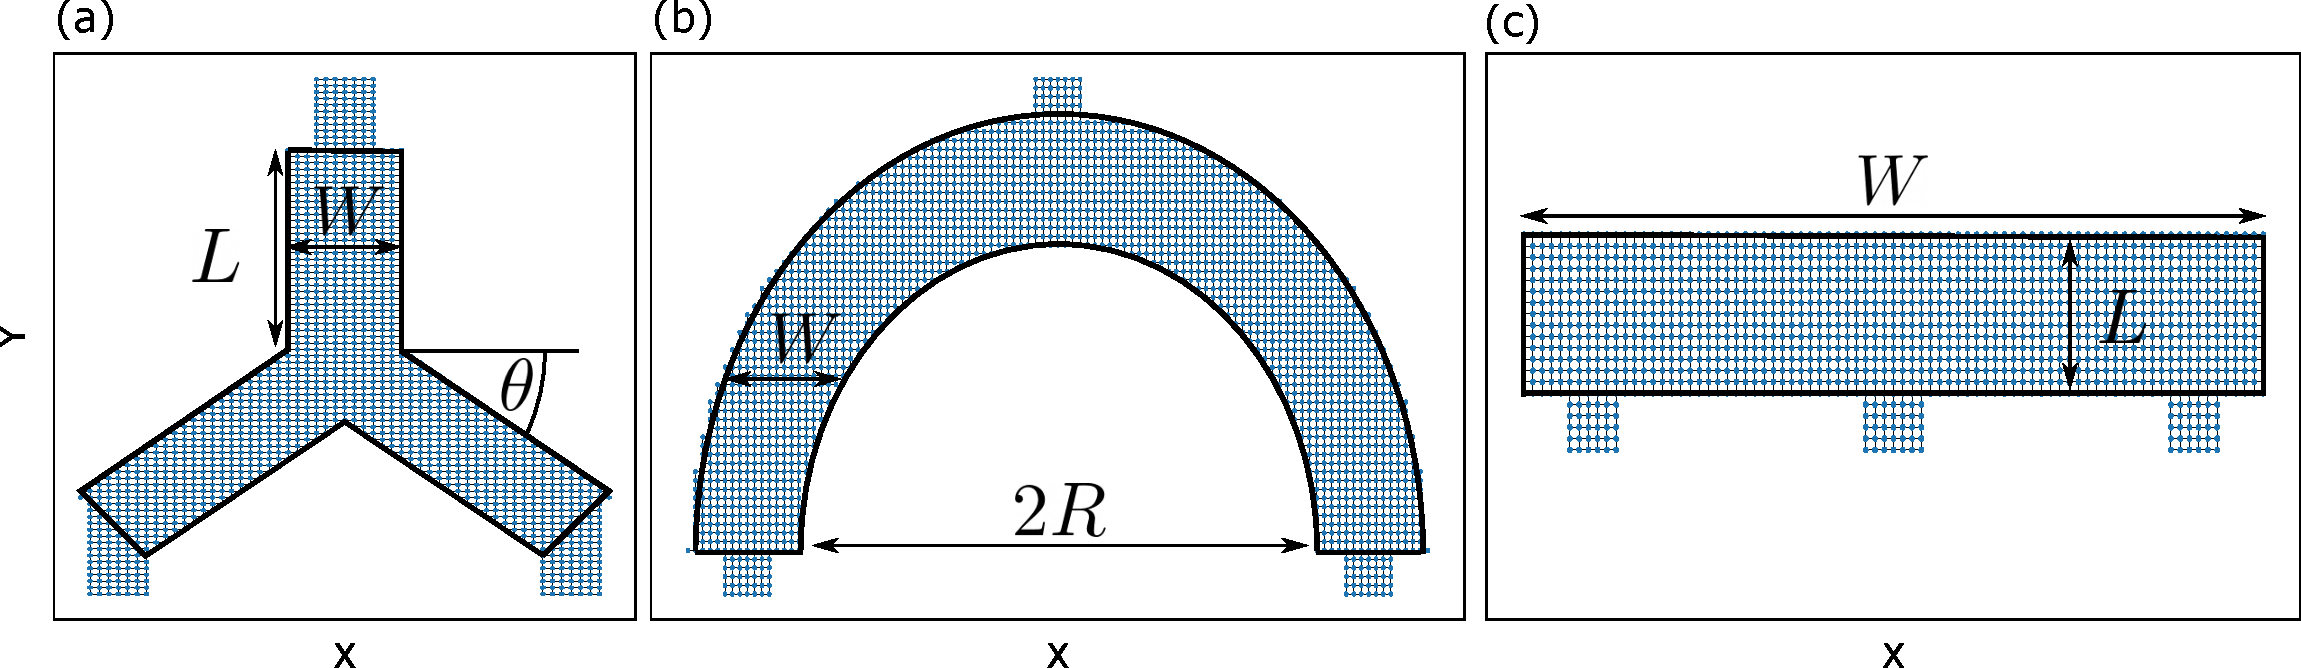
\includegraphics[width=0.9\linewidth]{figures/1d_cavities.pdf}
  \caption{Kwant systems describing the three quasi-1D cavities: (a) Y-shaped defined by three parameters: arms length and width, $L$ and $W$, and lateral arms angle $\theta$. (b) Half-ring defined by the radius $R$ and the width $W$. (c) Rectangular stripe defined by the length $L$ and width $W$.}
  \label{fig:1d}
\end{figure}

Consider a quasi-1D cavity with mirror symmetry around the $y$-axis.
The position of the three nanowires is fixed: one is attached at the center, and one at each end.
Consequently, the phase shift for the central MBS pairs is symmetric around $\pi$ as in Fig. \ref{fig:tj_example} (a).
Similarly, the coupling of the left-center MBS pair and center-right MBS pair is the same as in Fig. \ref{fig:tj_example} (b).
Under these constrains, we study how the geometry affects the coupling of the two different pairs.

We consider three cavity geometries:
In Fig. \ref{fig:1d} (a) one can observe a Y-shaped cavity. 
In Fig. \ref{fig:1d} (b) one can observe a half-ring stripe cavity with three nanowires attached in a fork-like geometry. 
In Fig. \ref{fig:1d} (c) one can observe a rectangular stripe cavity with three Majorana nanowires attached.

\subsection{Trijunction performance with respect to system size}

Initially, the overall size of the system is varied, and a transition from the small to the long junction regime is found for all geometries.
In Fig. \ref{fig:1d_results} one can observe the evolution of the largest resonance peak for each geometry as a function of the system size.

\begin{figure}[h!]
\centering
  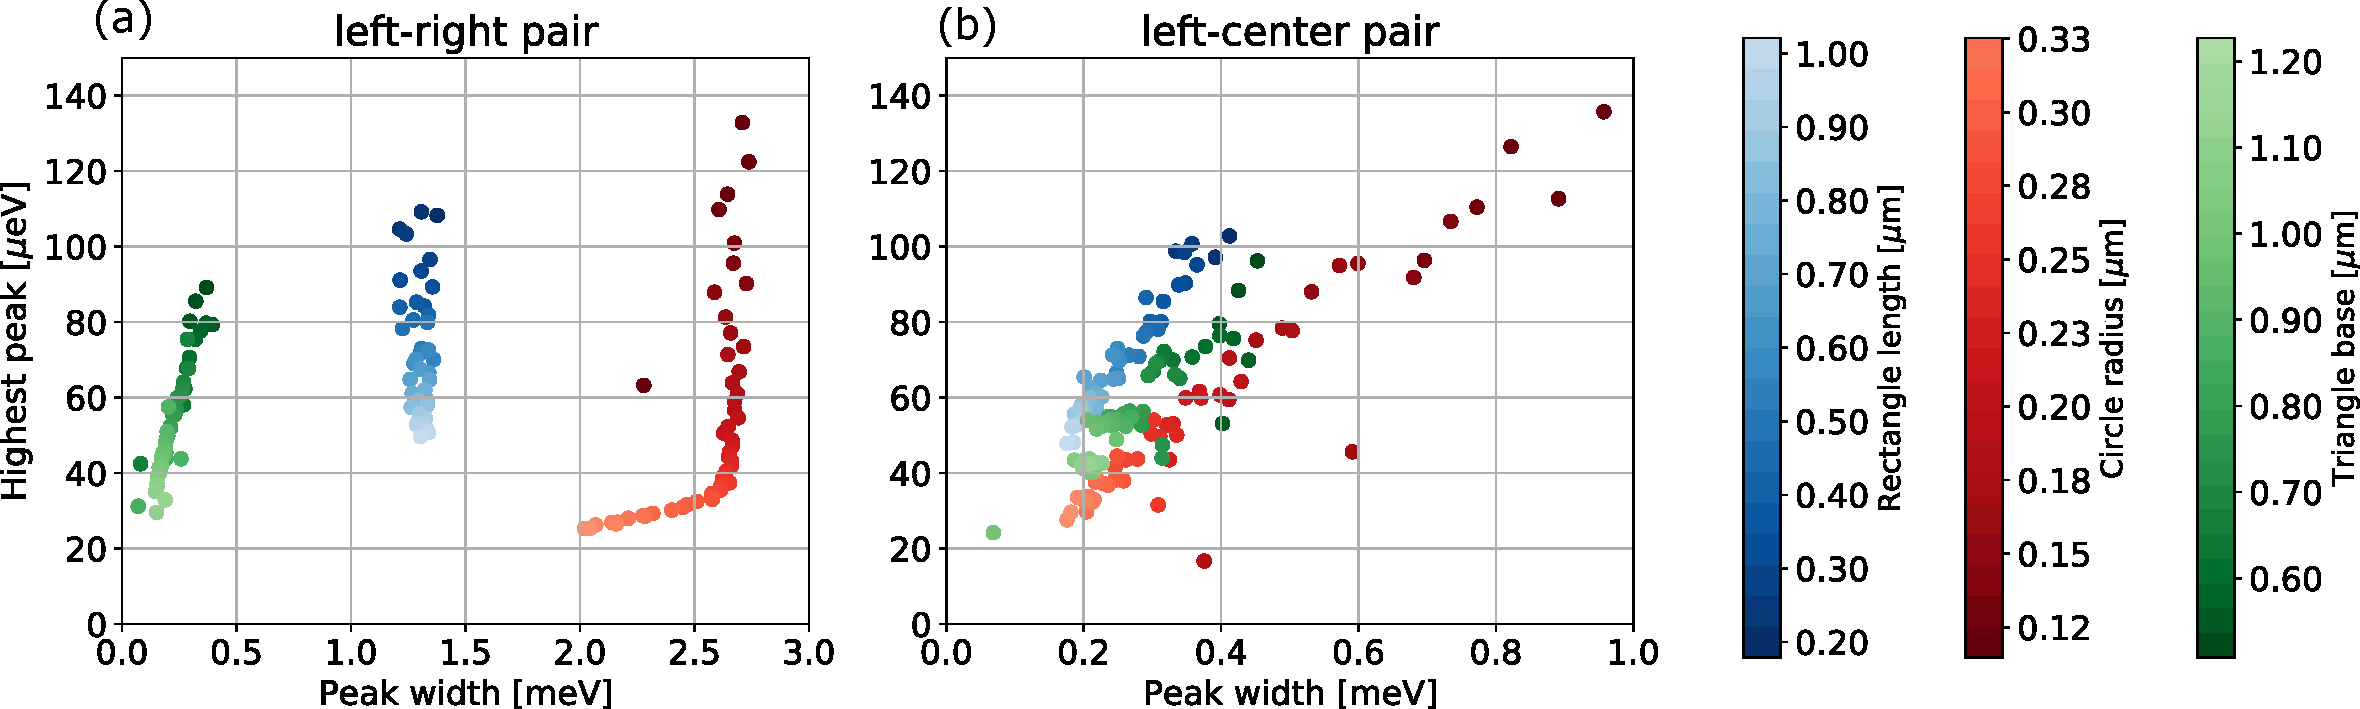
\includegraphics[width=\linewidth]{figures/couplings_1d.pdf}
  \caption{Geometrical dependence of the resonant coupling peaks for three quasi-1D geometries that correspond to each colorbar. The system is tuned to the lowest Majorana band. (a) Left-right MBS pair coupling. (b) Left-center MBS pair coupling.}
  \label{fig:1d_results}
\end{figure}

The coupling of the left and right MBS pair shows a clear geometrical dependence as can be observed in Fig. \ref{fig:1d_results} (a).
Each geometry occupies a separate region in the resonant height-width plane.
The ring cavity has the most robust resonant peaks.
For small $R$, the coupling is larger than any other geometry.
Similarly, the width is the largest, and it persists even for rings with diameter $1$ $\mu$m after which decays.
Then follows the stripe geometry that has approximately the same width for all considered geometries.
Finally, the Y-shaped cavity has overall the smallest resonant peak width. 

The coupling of the central MBS pairs, on the contrary, cannot be easily separated for each geometry.
Generally, one can see three diagonal stripes in Fig. \ref{fig:1d_results} (b) where the stripe geometry has the largest resonant peak height.
The peak width decreases as the size increase, and it has the same slope for all geometries.
Nevertheless, for sufficiently small sizes, the ring geometry has peak heights and widths larger than any other geometry.

We have found that there is systematic difference in the resonance peak width for different quasi-1D geometries.
A large coupling can be found for reasonably large devices, e.g. nanowire separation around $1$ $\mu$m.

\subsection{Resonant trapping}

\begin{figure}[h!]
\centering
  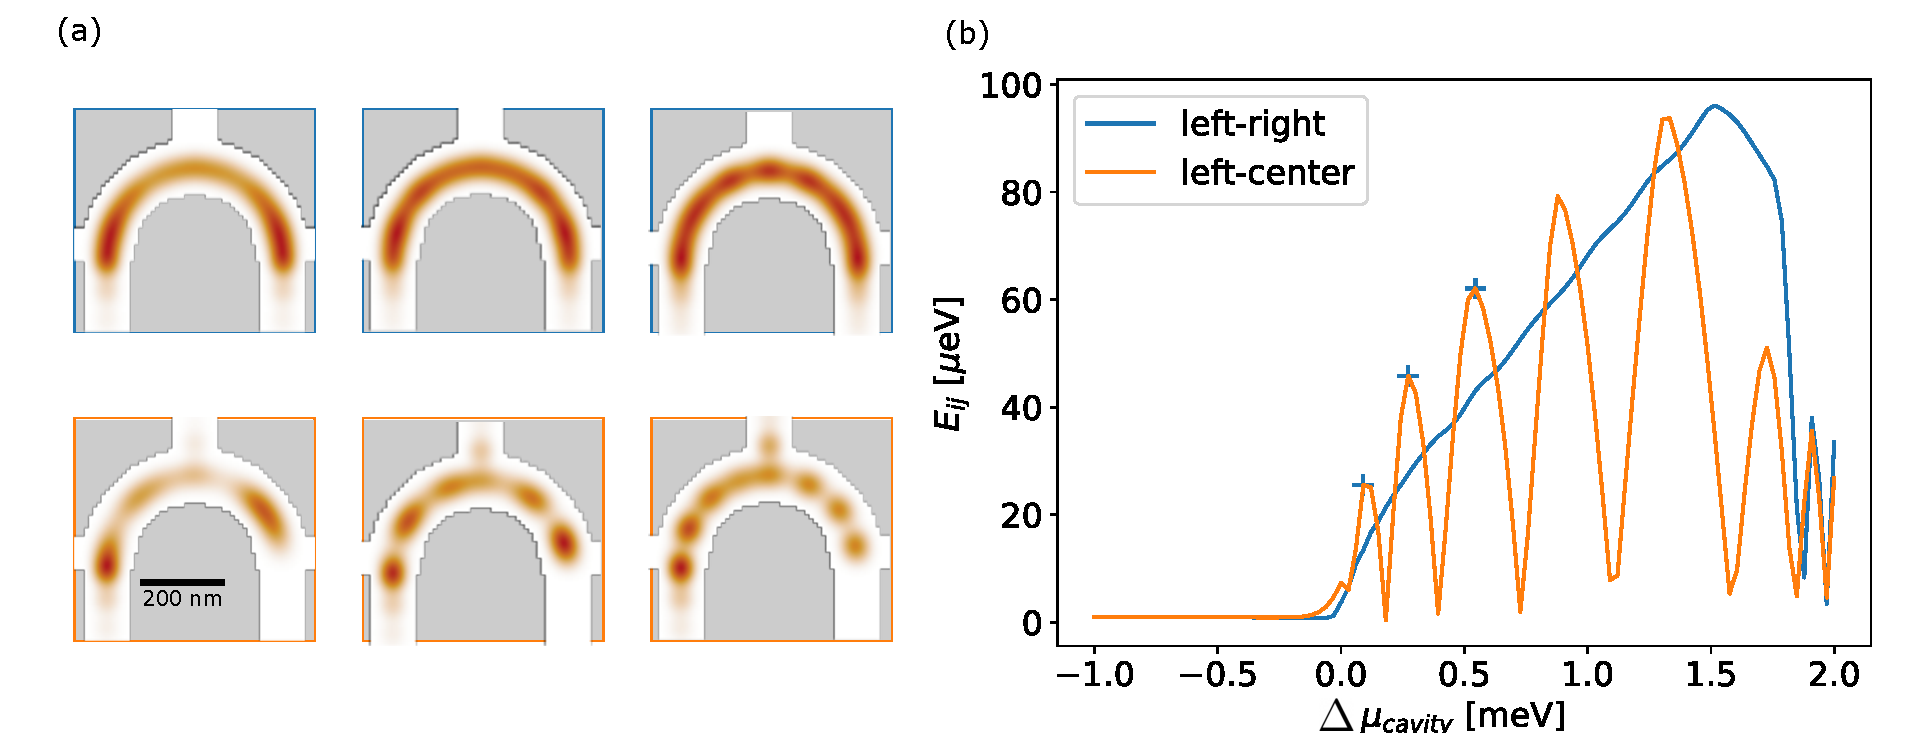
\includegraphics[width=\linewidth]{figures/resonant_trapping_ring.pdf}
  \caption{Spectra for a half-ring shaped cavity of width $W=110$ [nm] and radius $R=300$ [nm]. The system is tuned to the lowest Majorana band. (b) Coupling of each MBS pair. Center-right pair is the same curve as left-center pair. Crosses indicate the positions at where the wavefunction (a) are taken. The color of the frame in (a) corresponds each MBS pair in (b).}
  \label{fig:resonant_trapping}
\end{figure}

Consider the half-ring cavity.
When the left and right nanowires are close to the ends of the cavity, the MBS pair couple along a sequence of overlapping resonant states as can be seen in the blue line of Fig. \ref{fig:resonant_trapping} (a).
The cavity states interfere constructively and the coupling accumulates creating a single wide peak over the resonant region.
It depends crucially on having the lead states around all of the cavity wavefunction as can be seen in Fig. \ref{fig:resonant_trapping} (b).
This phenomena is known as \textit{resonant trapping} \cite{Nazmitdinov2001,Nazmitdinov2002}.

For the central pairs coupling, in contrast, a band of resonances cannot form since the cavity wavefunction is not fully enclosed.
When coupling the left and central MBS, the cavity region close to the right lead acts as a particle in a box with multiple individual levels that repel each other.
Consequently, we observe the orange line shown in Fig. \ref{fig:resonant_trapping} (a) where the resonant band is divided in individual resonances.

The difference when coupling multiple MBS pairs relies on the geometric configuration of the cavity wavefunctions and the MBS relative positions.
Then, one can explain the distribution of couplings observed in Fig. \ref{fig:1d_results}.
The left and right MBS in the ring and stripe geometry have an approximately constant and large widths over the different system sizes because cavity levels remain resonant.
On the other hand, the coupling of the central MBS pairs in any geometry has a much smaller width because some part of the wavefunction is not coupled.
Particularly, the Y-shaped junction has a small width for all pairs because no resonant trajectories can be created in such geometry.

\section{Two dimensional cavities}

\begin{figure}[h!]
\centering
  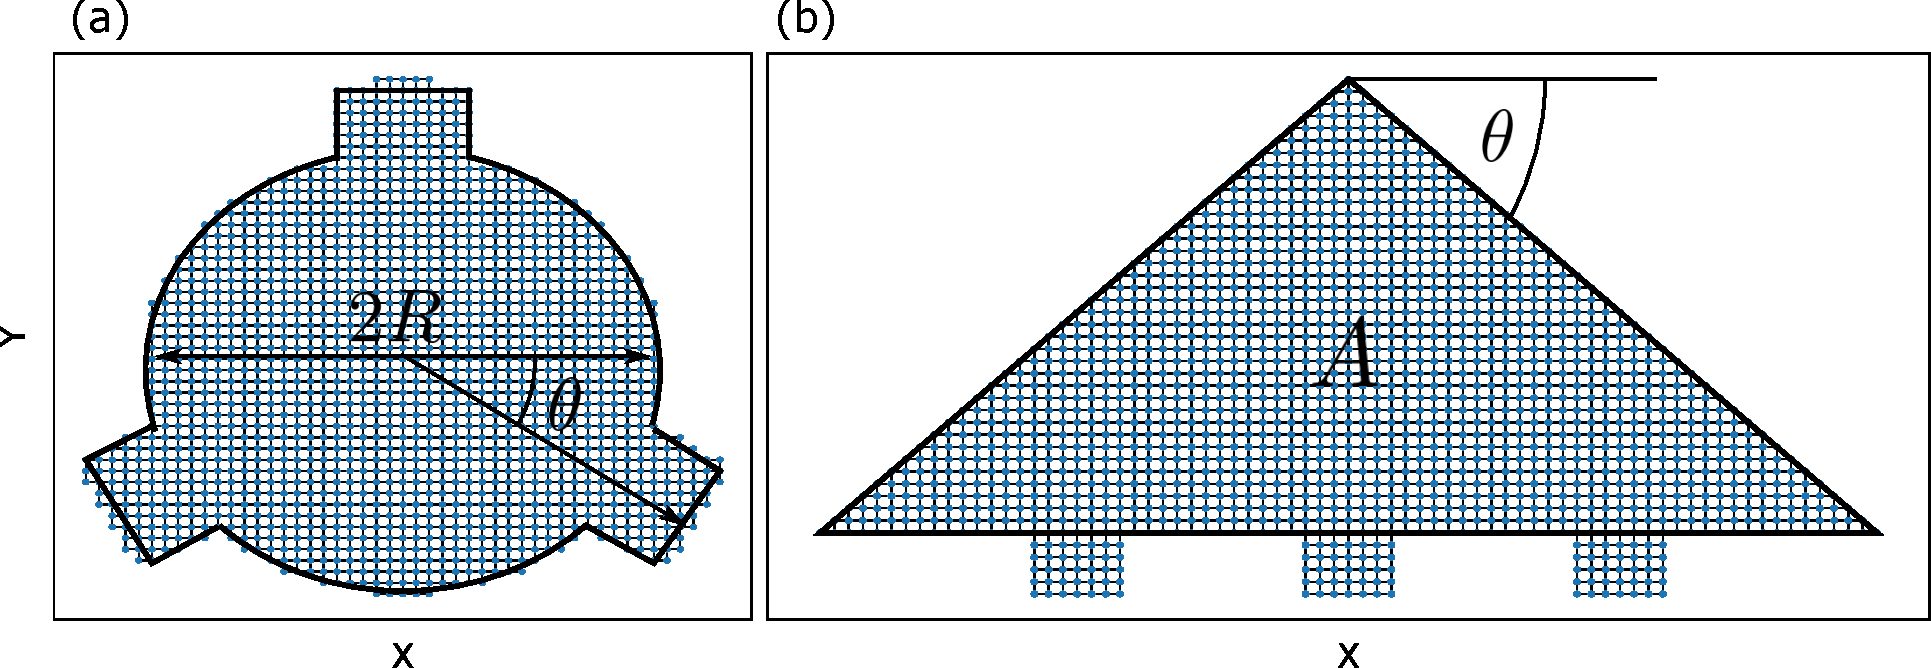
\includegraphics[width=0.9\linewidth]{figures/2d_cavities.pdf}
  \caption{(a) Kwant system of a circular shaped cavity. It is defined by the radius $R$ and the angle of the leads $\theta$. (b) Kwant system of a triangular shaped cavity. It is defined by the total area $A$ and the angle of the diagonal sides $\theta$.}
  \label{fig:2d}
\end{figure}

In a ballistic cavity, the motion of the electrons is determined by the shape of the cavity and leads.
The electrons follow semiclassical trajectories connecting different leads that can be identified as peaks in the conductance \cite{Wirtz1997}.
Following such intuition, we explore if changes in the geometry of a 2D cavity can be used to modulate the coupling of different MBS pairs.
Particularly, we explore how the angular dependence of the incoming modes, and internal angles of the cavity, influence the MBS coupling.

We consider three geometries:
In Fig. \ref{fig:2d} (a) one can observe a circular cavity with Majorana nanowires attached in a fork-like geometry.
In this geometry one can control the angle of the incoming MBS.
In Fig. \ref{fig:2d} (b) one can observe a triangular cavity with nanowires attached at the lower side.
In this geometry one can control the angle of MBS scattering within the cavity by changing the diagonal sides.
In order to explore to role of the positioning of the leads, we explore a variation of the triangular geometry with the central lead in the top side.
Lastly, we consider a rectangular geometry that can be created by extending the length of the stripe geometry shown in Fig. \ref{fig:1d} (c).

\subsection{Trijunction performance with respect to system size}

\begin{figure}[h!]
\centering
  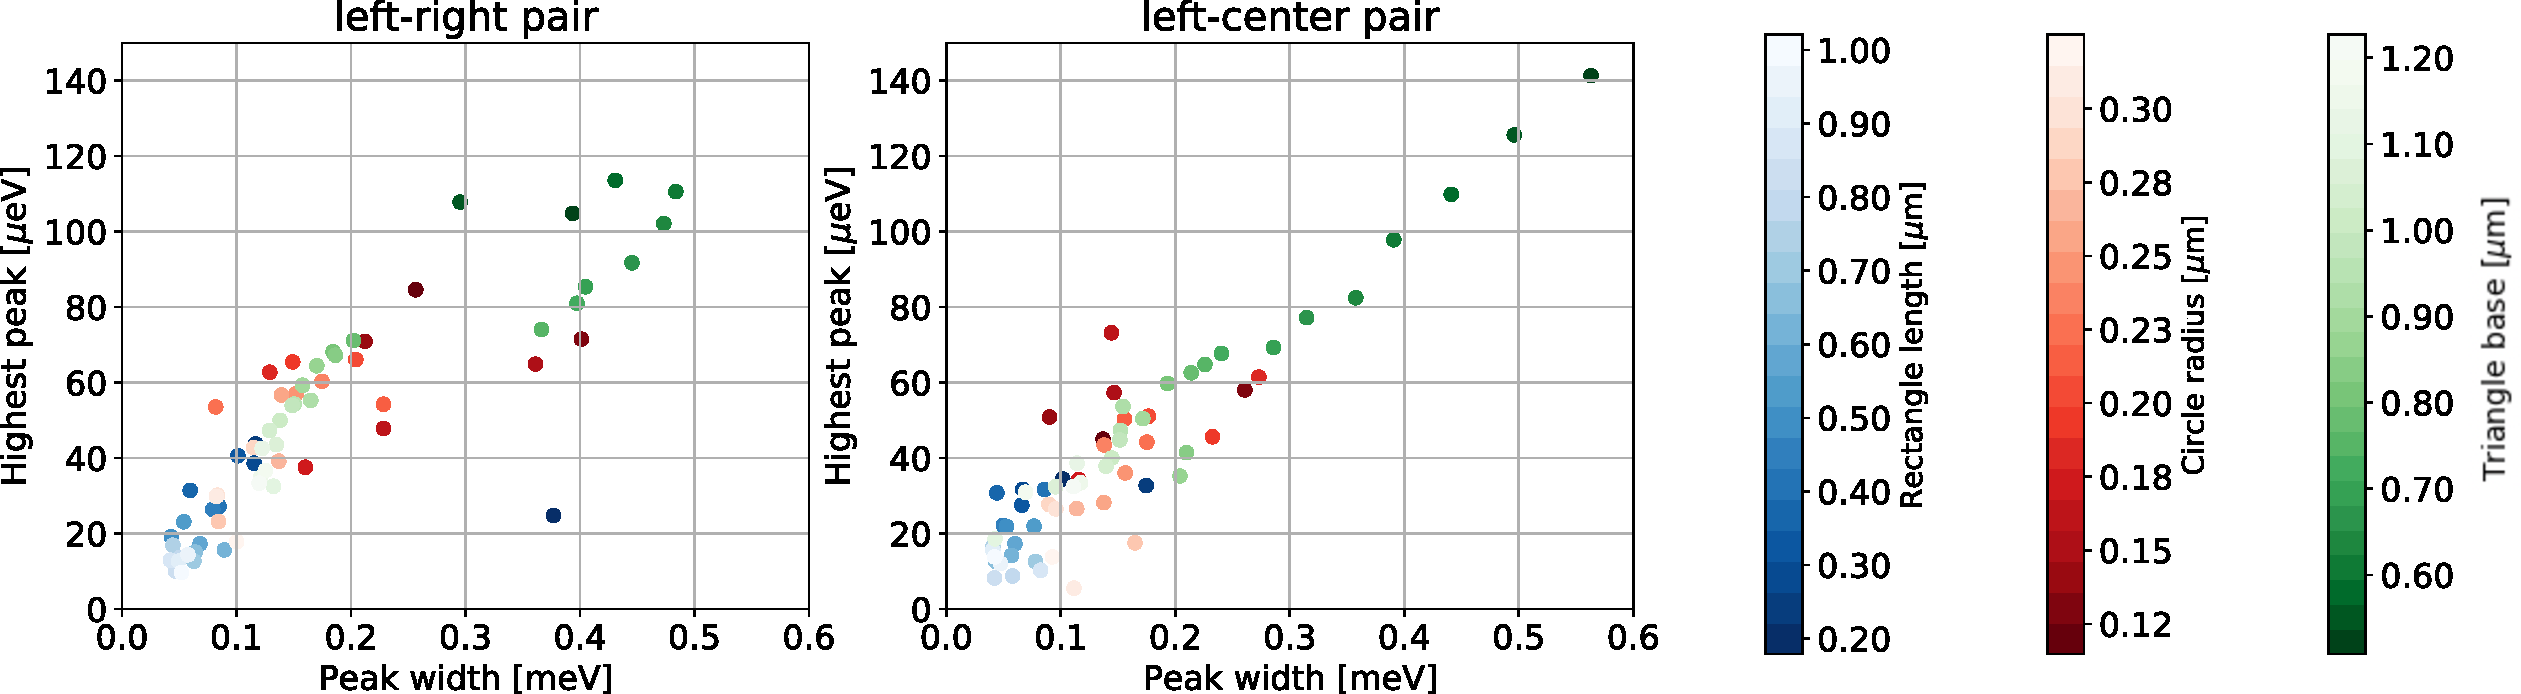
\includegraphics[width=\linewidth]{figures/couplings_2d.pdf}
  \caption{Size dependence of the three 2D geometries considered in this section corresponding to each colorbar. The system is tuned to the lowest Majorana band. The (a) left right and (b) left center largest resonant peaks are shown. The angle of all the cavities here is $\theta=\pi/4$.}
  \label{fig:2d_size_results}
\end{figure}

In Fig. \ref{fig:2d_size_results} one can observe the size dependence of the resonant peak for the three two-dimensional geometries considered.
Overall, there is no major distinction between the coupling of different pairs.
All couplings decays as the system size increases following a diagonal line in Fig. \ref{fig:2d_size_results} panels (a) and (b).
Nevertheless, the geometry dependence can be seen in three different regions along the diagonal.

On the rightmost region, one observes that the triangular geometry has the largest couplings and widths for small sizes.
Descending along the diagonal, the triangular and circular geometries overlap.
Remarkably, there is a significant size difference between them in the overlapping region, approximately $500$ nm.
Most of circular geometries are concentrated in this region.
At the bottom of the diagonal, one observes that the worst MBS couplings happen for rectangular geometries.

Unlike quasi-1D geometries, the size dependence 2D geometries considered does not have a clear boundary.
Nevertheless, a large coupling can be found for reasonably large devices in the case of the triangular cavity.

\subsection{Trijunction performance with respect to cavity angle}

\begin{figure}[h!]
\centering
  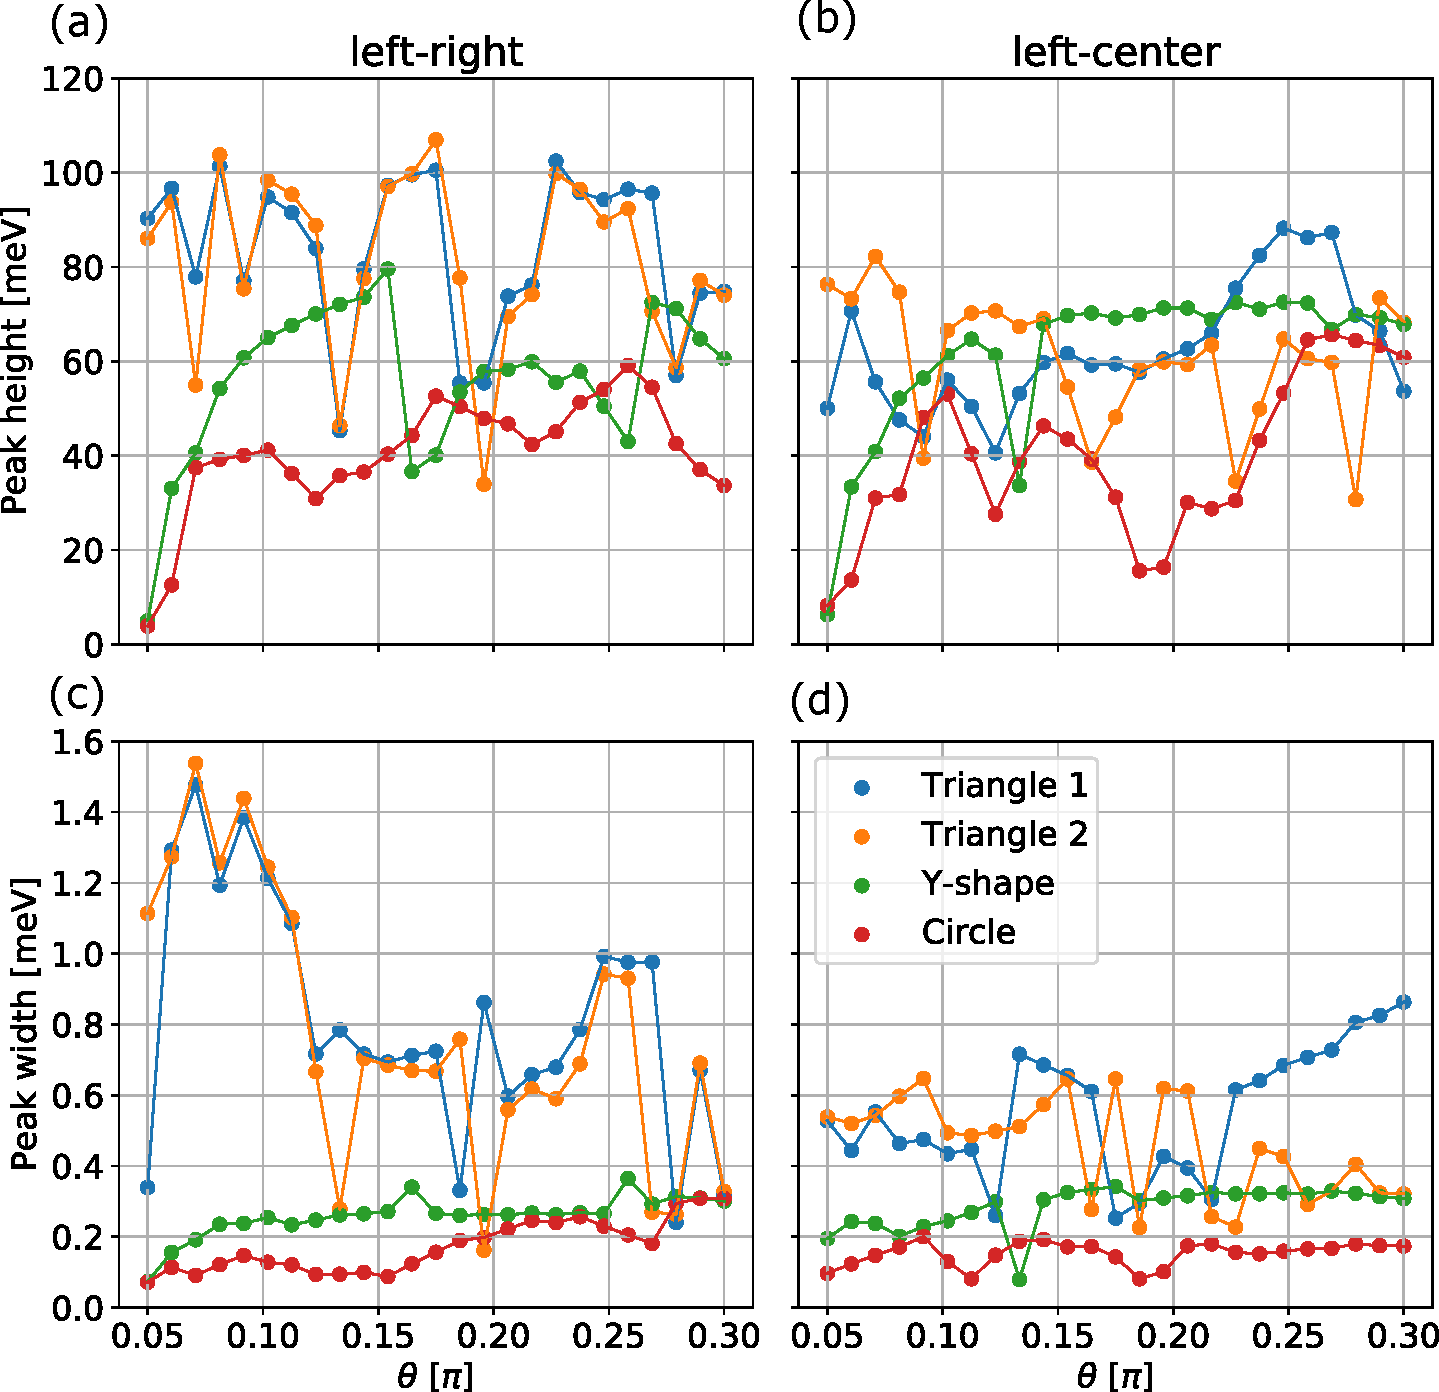
\includegraphics[width=0.78\linewidth]{figures/angles_height_width.pdf}
  \caption{Angular dependence of the resonant coupling peaks for four geometries with angle dependence. The system is tuned to the lowest Majorana band. Peak height and width for (a, c) left-right MBS pair and (b, d) left-center MBS pair coupling. The dimensions (base $\times$ height) of the triangle vary between $1 \times 0.15 $ $\mu$m for small angles up to $0.4 \times 0.5$ $\mu$m for large angles. The radius of the circular cavity is $R=250$ [nm]. The size of the Y-shaped cavity is similar to that of the triangular cavity.}
  \label{fig:angles_couplings}
\end{figure}

The angle is varied in two triangular cavities, one circular cavity, and the Y-shaped cavity.
The resulting coupling for each pair and geometry is shown in Fig. \ref{fig:angles_couplings}.
In Fig. \ref{fig:angles_couplings} (a) one can observe that there is a large variation of the peak height, yet there are angle ranges where the coupling stays approximately constant.
In Fig. \ref{fig:angles_couplings} (c) one can observe two different regions in the resonant peak width.
For small angles, the width is large, but as the angle increases the width drops.
In these two figures we observe a transition from the resonant trapping regime to the single resonance regime while maintaining an approximately constant peak height.
Note that for small angles the triangular cavity resembles a quasi-1D system.
By cutting the edges of the stripe geometry, the wavefunction concentrates around the center such that it is easily trapped between the left and right leads as observed in the blue curve of Fig. \ref{fig:triangle_transition} (a).
As the angle increases, the resonant band splits into several sub bands that contain a few resonances each as observed in Fig. \ref{fig:triangle_transition} (b).

The coupling of the left and central MBS pair for the triangular geometries shown in Fig. \ref{fig:angles_couplings} (b) and (d) shows no systematic behaviour.
Nevertheless, one observes in Fig.  \ref{fig:angles_couplings} (b) that the configuration with wires at the lower side (blue dots) has a maximum at large angles, while the configuration with wires at both sides has a maximum at small angles.
Furthermore, by comparing peak height around these two peak in Fig. \ref{fig:angles_couplings} (a) and (b), one observes that both are in the range $80-100$ $\mu$eV.
Therefore, there are two triangular configurations where the coupling of all pairs reaches a similar value.
Note, however, that the small angle configuration would be rather considered a quasi-1D system since the ratio between its dimensions.

\begin{figure}[h!]
\centering
  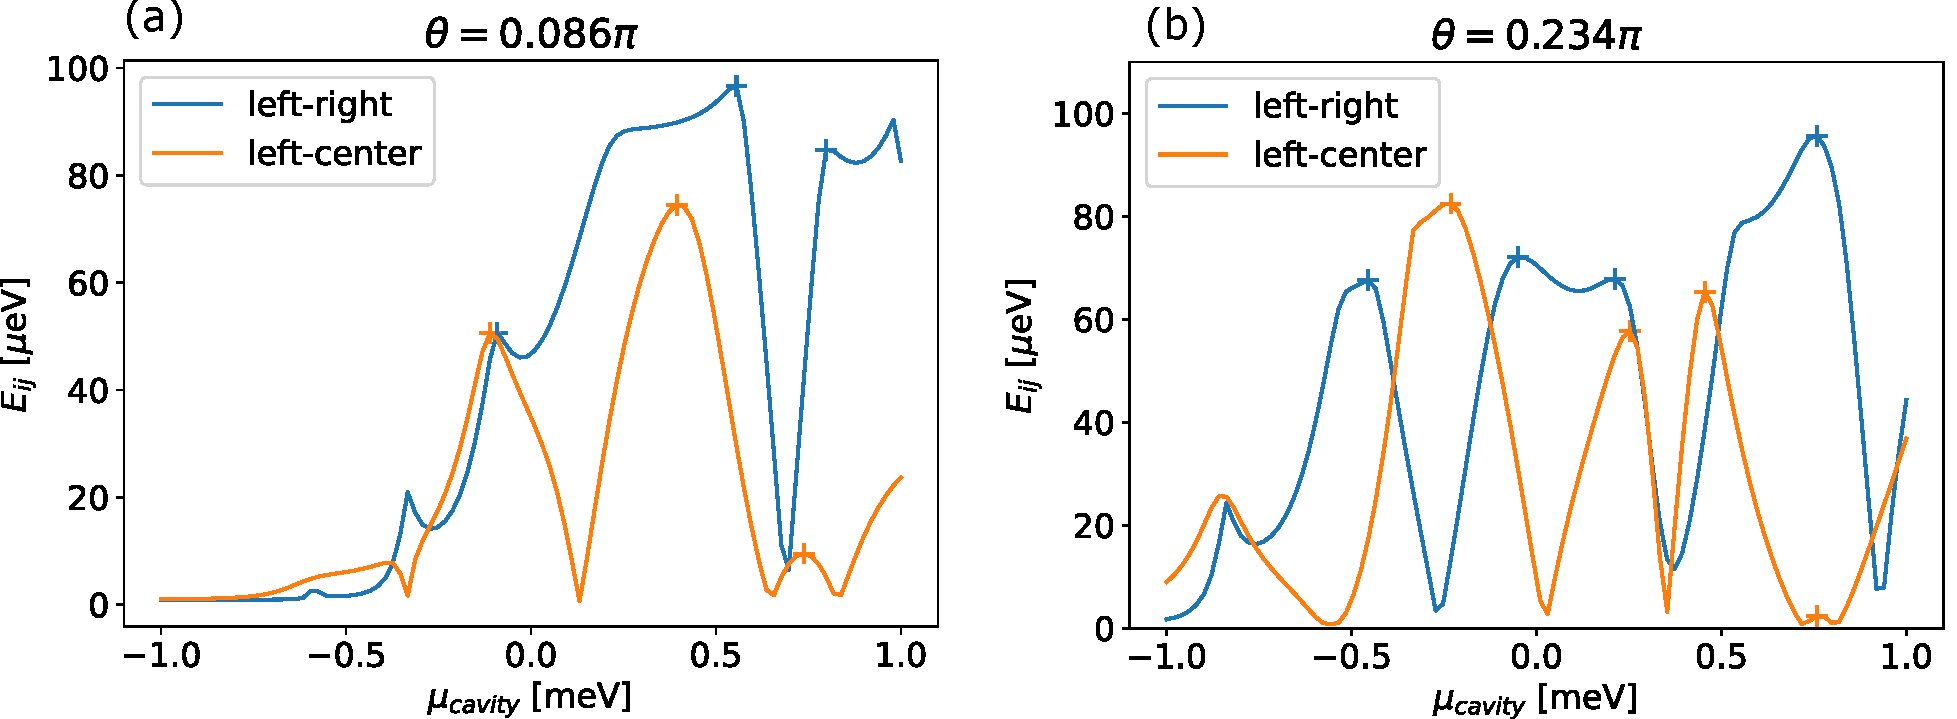
\includegraphics[width=0.8\linewidth]{figures/triangle_couplings.pdf}
  \caption{Coupling of triangular geometries with the central lead at the (a) top and (b) bottom sides.}
  \label{fig:triangle_transition}
\end{figure}

For the remaining geometries, there is indeed a modulation for the left and right MBS pairs.
The overall coupling is comparable to the triangular geometries, but the width is much smaller.
The left and central MBS coupling for the Y-shaped cavity converges to a peak height of about $70$ meV as the angle increases (see Fig. \ref{fig:angles_couplings} (c) green points).
The circular geometry shows that different angles enhance the coupling of different pairs as can be seen in the red lines.

The angular dependence does not show a systematic difference for the triangular geometries, but it does for the Y-shaped cavity.
However, for devices with similar size, the resonant peak height has a large difference between geometries, and the triangular geometry dominates.

\subsection{Majorana sub bands}

\begin{figure}[h!]
\centering
  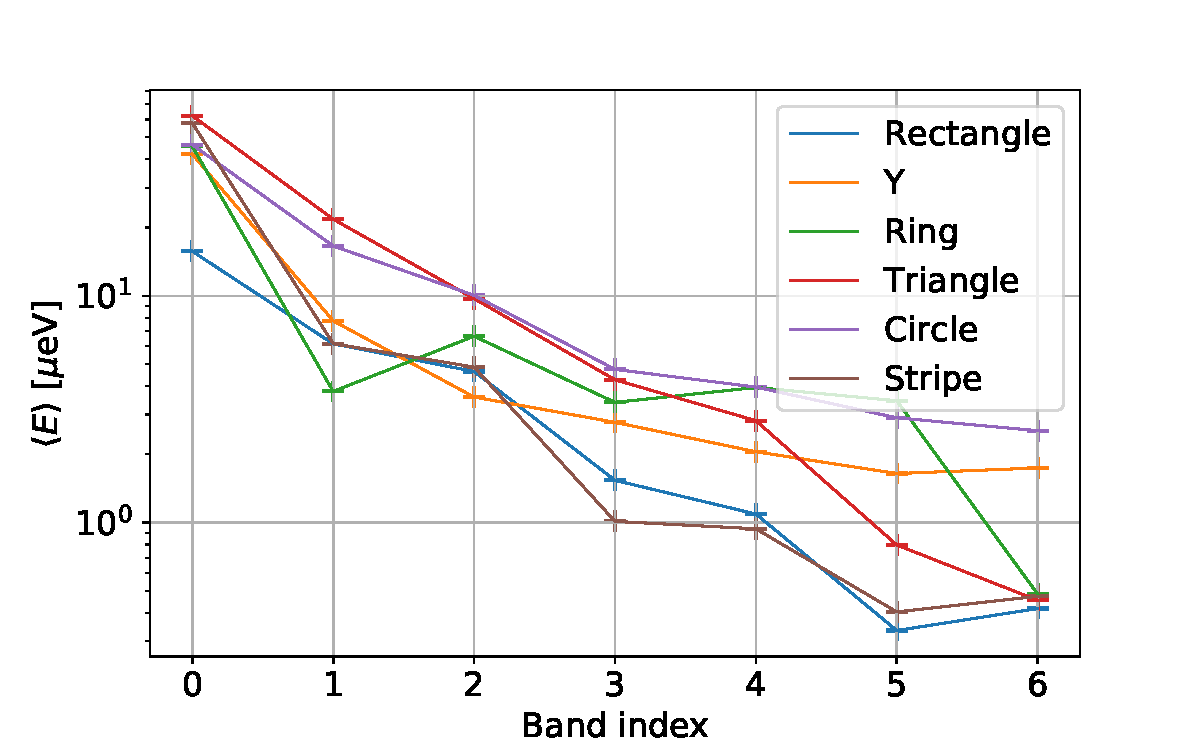
\includegraphics[width=0.6\linewidth]{figures/sub_bands_results.pdf}
  \caption{Mean geometry-pair coupling for all Majorana sub band and all geometries considered in this section. The geometry average is taken over the data shown in Fig. \ref{fig:2d_size_results}.}
  \label{fig:sub_bands}
\end{figure}

By tuning each nanowire sub band into the topological phase, we probe the momentum distribution of the cavity states.
In Fig. \ref{fig:sub_bands} one can observe the mean coupling for each band.
It has been averaged over all geometrical configurations and all MBS pairs since no clear distinction between them is found.

Overall, the coupling decays exponentially as the band index increases.
The decay is modulated by the geometry, but the trend holds in all cases.
There is, approximately, two order of magnitude decrease in the coupling from the lowest to the highest band.

The lowest band carries the largest coupling.
This allows us to infer that the momentum distribution of cavity states is dominated by low momentum states.
This behaviour is expected to change in the presence of disorder due to coupling of different momentum channels.
However, a precise quantitative description of the momentum profiles and the presence of disorder goes beyond the scope of this work.
\chapter{Gate defined triangular cavities}

\section{Gates configuration}
\begin{enumerate}
\item The triangular cavity is defined using electrostatic gates, and the potential in the 2DEG is found as the solution to the Poisson equation.
\item It is not clear if the geometric dependence holds in a real device where the boundaries of the system are not straight, but smooth following the potential landscape.
\item In contrast to a purely geometric model, changing a single gate has a non-local effect that affects other regions of the potential, possibly inducing unexpected behaviours.
\item The MBS coupling depends on the tradeoff between tunability and shape-resolution determined crucially by the position where the nanowires attach to the cavity.
\item Consider a material stack made by an InAs 2DEG with proximity induced superconductivity, and a set of metallic gates with an oxide layer in between.
\item There are three kinds of gates in this system: plunger gates and screen gates that control the shape of the cavity, and tunnel gates that control the coupling with the nanowires.
\item Devices with three nanowires at one side are larger than those with two because of the minimum separation between tunnel barriers which is required to have well defined coupling channels for each nanowire.
\end{enumerate}

\section{Device operation}
\subsection{Nanowire channels}
\begin{enumerate}
\item In order to have the minimum number of tunnable gates, each nanowire requires a tunnel barrier well separated from each other by fixed-voltage screen gates.
\item The operation point is below the first barrier level resonance in order to avoid interaction with spurious levels and keep a clean cavity dependence.
\item By controlling the tunnel gates height relative to the nanowire's potential, the tunnelling amplitude can be changed from the insulating regime to the strong coupling regime.
\item When the tunnel gates are far from each other, there is no crossed interaction between them, and they can be tunned symmetrically.
\item For closer tunnel gates, there's mutual interaction that modifies the barrier height, center and width, leading to a non-symmetric operational point.
\end{enumerate}
\subsection{Potential deformations}
\begin{enumerate}
\item While the left and right MBS coupling is optimal for a triangular cavity, the coupling of the central pairs is significantly smaller due to the large system size.
\item The triangular shape of the cavity is controlled by three gates, the plunger and the screen side gates, and can be deformed in order to probe modified shapes with increased couplings.
\item The coupling of the central pairs can be significantly increases by detunning the side screen gates and effectively creating smaller triangular cavities.
\item Potential deformations are not allowed in a geometry with the central wire attached to the top triangle vertex because the screen gates determine both the cavity shape and the barrier's positions.
\item Similarly, a configuration with nanowires attached to the diagonal sides would induce an irregularities along these sides that would significantly decrease the MBS coupling.
\end{enumerate}


\chapter{Conclusions}

In this work we have demonstrated that the question of designing an optimal trijunction of Majorana nanowires requires consideration of geometric, and electrostatic details.
We have not answered the question of what is the optimal geometry, but we have made progress by analysing different geometries in 1D and 2D.

We have found a systematic difference between different cavity geometries.
In quasi-1D cavities, there is a clear behaviour of the different geometries considered.
On the other hand, 2D systems show a complex behaviour where device size and shape influence the coupling and shape resolution.
Overall, the ring and the triangular geometry have the largest coupling in terms of resonance peak hight and width.

The implementation of a gate-defined trijunction requires a systematic tuning of the device.
We have found that the geometric description holds for two-dimensional shapes.
However, as the system size decreases, electrostatics dominate over the purely geometrical effects.
Nevertheless, a gate-defined shape can be further optimised by deforming the shape of the cavity in a new gate voltage regime.

This work can be extended in three possible ways:
On the one hand, further geometry analysis can be used to find the optimal cavity shape that will be later implemented with an electrostatic model.
On the other hand, include a measurement protocol that allows to measure the state encoded by the MBS.
This is a necessary ingredient in order to design a Majorana qubit.
Finally, both previous approaches require the inclusion of disorder effects to have a realistic description

The implementation of a gate-defined ring geometry remains as an open question.
The main problem that we found with this geometry is that the coupling between different pairs is highly asymmetric due to resonant trapping.
Nevertheless, this problem can be circumvent by defining multiple regions along the ring that can be activated or depleted depending on the pair to couple.

Another possible extension is to implement an optimisation algorithm that determines the optimal shape of the cavity.
To consider all pairs simultaneously, one can optimise the minimum coupling.
This thesis can be used to establish the constraints on the algorithm, such as device size and nanowire separation.
Once the shape is found, an electrostatic implementation is required to determine the feasibility of such result.


%% Use letters for the chapter numbers of the appendices.
\bibliography{chapters/biblio}
\end{document}

